\documentclass{report}

\input{~/latex/template/preamble.tex}
\input{~/latex/template/macros.tex}

\title{\Huge{Chapter 3 Notes}}
\author{\huge{Matt Warner}}
\date{\huge{}}
\pagestyle{fancy}
\fancyhf{}
\rhead{Math 211 - Calculus For Business \& Social Science}
\lhead{\leftmark}
\cfoot{\thepage}
% \usepackage[default]{sourcecodepro} \usepackage[T1]{fontenc}
\usepackage{pgfplots}
\usetikzlibrary{calc}
\pgfplotsset{compat=newest}
\pgfpagesdeclarelayout{boxed}
{
  \edef\pgfpageoptionborder{0pt}
}
{
  \pgfpagesphysicalpageoptions
  {%
    logical pages=1,%
  }
  \pgfpageslogicalpageoptions{1}
  {
    border code=\pgfsetlinewidth{1.5pt}\pgfstroke,%
    border shrink=\pgfpageoptionborder,%
    resized width=.95\pgfphysicalwidth,%
    resized height=.95\pgfphysicalheight,%
    center=\pgfpoint{.5\pgfphysicalwidth}{.5\pgfphysicalheight}%
  }%
}

\pgfpagesuselayout{boxed}

\begin{document}
  \maketitle
  \section*{3.1 - Using First Derivaties to Classify Maximum and Minimum Values}
  \bigbreak \noindent \bigbreak \noindent
  \hrule
  \bigbreak \noindent
  \vspace{-3mm}\subsection*{Increasing and Decreasing Functions}
  \bigbreak \noindent
  If the graph of a function rises from left to right over an interval $I$, the function is said to be increasing on, or over, $I$.
  \bigbreak \noindent
  If the graph drops from left to right, the function is said to be decreasing on, or over, $I$.
  \begin{figure}[ht]
  \centering
  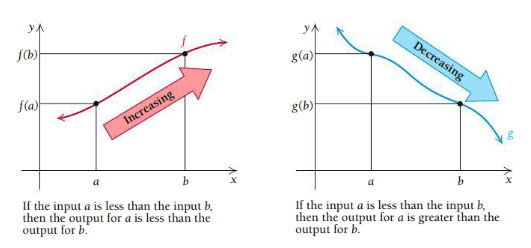
\includegraphics[width=0.65\textwidth]{  /home/mattw/niu/Math211/latexdocs/figures/paste.png}
  \end{figure}
\bigbreak \noindent
We can define these concepts as follows.
\begin{mdframed}
  \vspace{2mm}

  A function $f$ is \textbf{increasing} over $I$ if, for every $a$ and $b$ in $I$, 
  $$ \text{if } a < b, \ \ \ \text{then } f(a) < f(b)$$
  A function $f$ is \textbf{decreasing} over $I$ if, for every $a$ and $b$ in $I$,
  $$ \text{if } a < b, \ \ \ \text{then } f(a) > f(b)$$
\end{mdframed}
\bigbreak \noindent
The above definitions can be restated in terms of slopes of secant lines
\bigbreak \noindent
\hspace{35mm}Increasing: $\dfrac{f(b) - f(a)}{b - a} > 0$ \hspace{20mm} Decreasing: $\dfrac{f(b) -f(a)}{b - a} < 0$
\begin{figure}[ht]
\centering
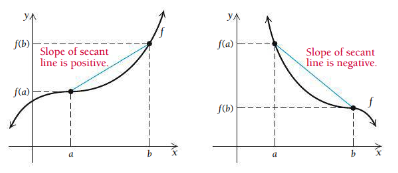
\includegraphics[width=0.65\textwidth]{ /home/mattw/niu/Math211/latexdocs/figures/second.png}
\end{figure}
\bigbreak \noindent
Since the derivative of a function tells us the slope of the tangent line to $f$ at any input x, we can also define an increasing or decreasing function using the derivative
\pagebreak
\thm{}{
  Let $f$ by differentiable over an open interval $I$
  \bigbreak \noindent
  If $f'(x) > 0$ for all x in $I$, then $f$ is increasing over $I$ 
  \vspace{2mm}

  If $f'(x) < 0$ for all $x$ in $I$, then $f$ is decreasing over $I$
}
\bigbreak \noindent
Theorem 0.1 is illustrated in the following graph of
$$ f(x) = \dfrac{1}{3}x^{3} - x + \dfrac{2}{3}$$
\begin{figure}[ht]
    \centering
    \incfig[1]{trialsiz}
    %\caption{trialsiz}
    %\label{fig:trialsiz}
\end{figure}
\bigbreak \noindent
Note in the graph above that x = -1 and x = 1 are not included in any interval over which the function is increasing or decreasing. These values are examples of \textit{critical values}
\bigbreak \noindent
\subsection*{Critical Values}
Consider the following graph
\begin{figure}[ht]
\centering
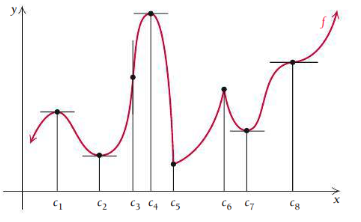
\includegraphics[width=0.5\textwidth]{ /home/mattw/niu/Math211/latexdocs/figures/critical.png }
\end{figure}
\bigbreak \noindent
Note the following
\begin{enumerate}
  \item $f'(x) = 0 \text{ for } x = c_1, c_2, c_4, c_7, \text{and }  c_8$. That is, the tangent line to the graph is horizontal at these values.
  \item $f'(x)$ does not exist for $ x = c_3, c_5$, and $C_6$. The tangent line is vertical at $c_3$, and there are corners at both $c_5$ and $c_6$.
\end{enumerate}
\pagebreak
\begin{mdframed}
  A \textbf{critical value}  of a function $f$ is any number $c$ in the domain of $f$ for which the tangent line at $(c,f(c))$ is \textbf{horizontal} or for which the derivative does not exist.
  \bigbreak \noindent
  That is, $c$ is a critical value if $f(c)$ exists and
  $$ f'(c) = 0 \ \ \ \text{or} \ \ \ f'(c) \text{ does not exist}$$
If $c$ is a critical value of a function $f$, then $(c,f(c))$ is a \textbf{critical point}
\end{mdframed}
Thus, in the graph of $f$ above:
\begin{itemize}
  \item $c_1, c_2,c_4,c_7,c_8$ are critical values because $f'(c) = 0$ for each value 
  \item $c_3,c_5,c_6$ are critical values because $f'(c)$ does not exist for each value
  \bigbreak \noindent
\end{itemize}
  \nt{
    A continuous function can change from increasing to decreasing or from decreasing to increasing \textbf{only} at a critical value.
  }
  \bigbreak \noindent
  \hrule
  \bigbreak
  \subsection*{Finding Relative Maximum and Minimum Values}
  Now consider a graph with ``peaks'' and ``valleys'' at $x = c_1, c_2, c_3, c_4$, and $c_5$
  \begin{figure}[ht]
  \centering
  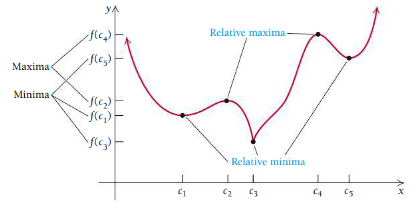
\includegraphics[width=0.5\textwidth]{ /home/mattw/niu/Math211/latexdocs/figures/peaks.png }
  \end{figure}
  \bigbreak \noindent
  Here, $f(c_2)$ and $f(c_4)$ are each an example of a \textbf{relative}, or \textbf{local, maximum}, and $f(c_1), f(c_3)$, and $f(c_5)$ are each an example of a \textbf{relative}, or \textbf{local minimum}.
  \bigbreak \noindent
  Collectively, maximum and minimum values are called \textbf{extrema}
  \nt{
  Note that it is possible for a relative minimum to be greater than a relative maximum.
  \bigbreak \noindent
  For example, $f(c_5) > f(c_2)$ in the graph in the next page.
  \bigbreak \noindent
  Also note that x-values at which a continuous function has relative extrema are those values for which the derivative is 0 or for which the derivative does not exist - the critical values
  }
  \pagebreak
  \thm{}{
    If a function $f$ has a relative extreme value $f(c)$ on an open interval, then $c$ is a critical value, and
    $$ f'(c) = 0 \ \ \ \text{or } \ \ f'(c) \text{ does not exist}$$
  }
\section*{Relative Extreme Points}

A relative extreme point, \( (c, f(c)) \), is higher or lower than all other points over an open interval containing \( c \).

\subsection*{Relative Minimum Point}

A relative minimum point, \( (c, f(c)) \), is lower than all other points over an open interval containing \( c \). Such a point has a \( y \)-value that is less than those of a neighborhood of points to the left and right of \( c \).

\subsection*{Relative Maximum Point}

Similarly, a relative maximum point, \( (c, f(c)) \), is higher than all other points over an open interval containing \( c \). This maximum point has a \( y \)-value that is greater than those of a neighborhood of points to the left and right of \( c \).

\textbf{Note:} In the preceding graph, \( (c_1, f(c_1)), (c_3, f(c_3)) \), and \( (c_5, f(c_5)) \) are all relative minimum points. Similarly, \( (c_2, f(c_2)) \) and \( (c_4, f(c_4)) \) are both relative maximum points.

\section*{Theorem 2}

\textit{Theorem 2 is useful and important to understand.} It states that to find relative extrema, we need only consider inputs for which the derivative is 0 or for which the derivative does not exist. Each critical value is a candidate for a value where a relative extremum might occur.

However, Theorem 2 does not guarantee that every critical value will yield a relative maximum or minimum. For instance, consider the graph of
\[
f(x) = (x-1)^3 + 2
\]
shown on the left. Note that:
\[
f'(x) = 3(x-1)^2 \quad \text{and} \quad f'(1) = 3(1-1)^2 = 0
\]
Thus, \( c = 1 \) is a critical value, but \( f \) has no relative maximum or minimum at that value. In fact, this function has no extrema anywhere.
\vspace{2mm}

\noindent Theorem 2 does guarantee that if a relative maximum or minimum occurs, then the first coordinate of that extremum is a critical value.
\bigbreak \noindent
The following graph leads us to a test.
\begin{figure}[ht]
\centering
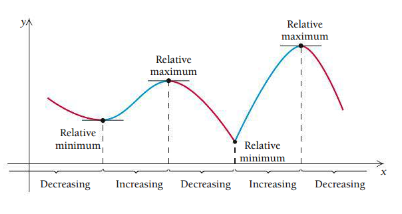
\includegraphics[width=0.58\textwidth]{ /home/mattw/niu/Math211/latexdocs/figures/test.png}
\end{figure}

\pagebreak
\begin{mdframed}
  \vspace{1.5mm}

Note that at a critical value where there is a relative minimum, the function $f$ is \textbf{decreasing} on the left of the critical value and \textbf{increasing} on the right.
\bigbreak \noindent
At a critical value where there is a relative maximum, the function $f$ is \textbf{increasing} on the left of the critical value and \textbf{decreasing} on the right. In both cases, the derivative changes signs on either side of the critical value.
\vspace{1.5mm}
\end{mdframed}
\bigbreak \noindent \bigbreak \noindent \bigbreak \noindent \bigbreak \noindent 
\begin{figure}[ht]
\centering
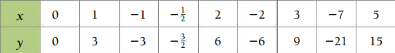
\includegraphics[width=0.9\textwidth]{ /home/mattw/niu/Math211/latexdocs/figures/table.png }
\end{figure}

\pagebreak
\noindent
Derivatives can tell us when a function is increasing or decreasing. This leads us to the First-Derivative Test.
\thm{}{
  For any continuous function $f$ that has exactly one critical value $c$ in an open interval $(a,b)$
  \bigbreak \noindent
  \textit{\textbf{F1.}} $f$ has a relative minimum at $c$ if $f'(x) < 0$ on $(a,c)$ and $f'(x) > 0$ on $(c,b)$. That is, $f$ is decreasing to the left of $c$ and increasing to the right of $c$
  \bigbreak \noindent
  \textit{\textbf{F2}} $f$ has a relative maximum at $c$ if $f'(x) > 0$ on ($a,c$) and $f'(x) < 0$ on ($c,b$). That is, $f$ is increasing to the left of $c$ and decreasing to the right of $c$
  \bigbreak \noindent
  \textit{\textbf{F3}} $f$ has neither a relative maximum nor a relative minimum at $c$ if $f'(x)$ has the same sign on $(a,c)$ as on $(c,b)$
  \bigbreak \noindent
  We can use the First-Derivative Test to find relative extrema.
}
\q
Consider the function $f$ given by
$$ f(x) = 4x^3 - 9x^2 - 30x + 25$$
\bigbreak \noindent
\textbf{Find any relative exterma}
\bigbreak \noindent
\textit{\textbf{Find the derivative}}

$$ \frac{d}{dx}[4x^3] - \frac{d}{dx}[9x^2] - \frac{d}{dx}[30] + \frac{d}{dx}[25]$$

$$ f'(x) = 12x^2 - 18x -30$$
\textit{\textbf{set f'(x) = 0}}

$$ 12x^2 -18x - 30 = 0$$
\textit{\textbf{divide both sides by 6}}
$$ 2x^2 - 3x -5 = 0$$
$$ (x+1)(2x-5) = 0$$
$$ x = -1 \ \ \ \ or \ \ \ \ x = \dfrac{5}{2}$$
The critical values are -1 and $\dfrac{5}{2}$. Since it is at these values that a relative maximum or minimum might exist, we examine the sign of the derivative on the intervals
$$ (-\infty, -1), (-1,\dfrac{5}{2}), (\dfrac{5}{2}, \infty)$$
To do so, we select a convenient test value in each interval and evalulate f'(x). 
\bigbreak \noindent
\textit{\textbf{Let's use the values: -2, 0, 4}}
$$ f'(-2) = 54$$
$$f(0) = -30$$
$$ f(4) = 90$$
\textit{\textbf{Result:}} \\

\noindent $f$ is increasing on $(-\infty, -1)$ \\
$f$ is decreasing on $(-1, \dfrac{5}{2})$ \\
$f$ is increasing on $(\dfrac{5}{2}, \infty)$ 
\bigbreak \noindent
By the First-Derivative Test, $f$ has a relative maximum at $x = -1$ and a relative minimum at $ x=\dfrac{5}{2}$
\bigbreak \noindent
The value of the relative maximum is given by
$$ f(-1) = 4(-1)^3 - 9(-1)^2 - 30(-1) + 25$$
$$ f(-1) = 42 $$
The value of the relative minimum is given by
$$ f(\frac{5}{2}) = 4(\frac{5}{2})^3 - 9(\frac{5}{2})^2 - 30(\frac{5}{2}) + 25$$
$$ f(\frac{5}{2}) = -\dfrac{175}{4} $$
\bigbreak \noindent
Thus, there is a relative maximum point at $(-1,42)$ and a relative minimum point at $(\frac{5}{2}, -\frac{175}{4})$
\bigbreak \noindent
\begin{center}
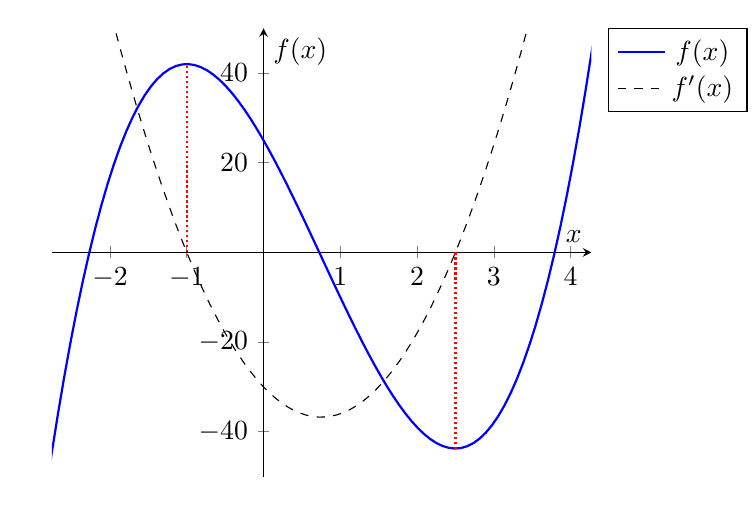
\begin{tikzpicture}
    \begin{axis}[
        axis lines = middle,
        xlabel = \(x\),
        ylabel = \(f(x)\),
        domain=-3:5,
        samples=100,
        ymin=-50,
        ymax=50,
        legend pos=outer north east,
    ]
    
    % Plotting f(x)
    \addplot[color=blue, thick]{4*x^3 - 9*x^2 - 30*x + 25};
    \hspace{3mm}\addlegendentry{\(f(x)\)}
    % Plotting f'(x)
    \addplot[color=black, dashed]{12*x^2 - 18*x - 30};
    \addlegendentry{\(f'(x)\)}
    % Marking and drawing vertical dashed lines for the critical points
    \draw [densely dotted, red, thick] (axis cs: -1,0) -- (axis cs: -1,{4*(-1)^3 - 9*(-1)^2 - 30*(-1) + 25});
    \draw [densely dotted, red, thick] (axis cs: 5/2,0) -- (axis cs: 5/2,{4*(5/2)^3 - 9*(5/2)^2 - 30*(5/2) + 25});
    \end{axis}
\end{tikzpicture}
\end{center}
\bigbreak \noindent
\nt{
  Note that $f'(x) = 0$ where $ f(x)$ has relative extrema. We summarize the behavior of this function by noting where it is increasing or decreasing and by characterizing its critical points
  \bigbreak \noindent
  \begin{itemize}
    \item $f$ is increasing over the interval $(-\infty, -1$) 
    \item $f$ has a relative maximum point at $(-1,42)$
    \item $f$ is decreasing over the interval $(-1,\dfrac{5}{2})$
    \item $f$ has a relative minimum point at $(\dfrac{5}{2}, -\dfrac{175}{4})$
    \item $f$ is increasing over the interval $(\dfrac{5}{2}, \infty)$
  \end{itemize}
}
\bigbreak \noindent
To use the first derivative for graphing a function $f$
\begin{enumerate}
  \item Find all critical values by determining where $f'(x)$ is 0 and where $f'(x)$ is undefined (but $f(x)$ is defined). Find $f(x)$ for each critical value
  \item Use the critical values to divide the x-axis into intervals and choose a test value in each interval
  \item Find the sign of $f'(x)$ for each test value chosen in step 2, and use this information to determine where $f$ is increasing or decreasing and to classify any extrema as relative maxima or minima
  \item Plot some additional points and sketch the graph
\end{enumerate}

\pagebreak
\q
Find the relative extrema and sketch the graph of the function $f$ given by
$$ f(x) = 2x^3  - x^4$$
\textit{\textbf{We first need to take the derivative}}
$$ f'(x) = \frac{d}{dx}2x^3 - \frac{d}{dx}x^4$$
$$ f'(x) = 6x^2 - 4x^3$$
\textit{\textbf{Find the critical values}}

$$ 6x^2 - 4x^3$$
$$ = 2x(3-2x)$$
$$ 2x^2 = 0 \ \ \ \ 3 - 2x = 0$$
$$ x = 0 \ \ \ \ x = \dfrac{3}{2}$$
\textit{\textbf{So, the intervals are}}

$$ (-\infty,0), \ \ \ (0,\dfrac{3}{2}), \ \ \ (\dfrac{3}{2}, \infty)$$
\bigbreak \noindent
\textit{\textbf{Choose test values within the intervals to see where its increasing / decreasing}}
$$(-\infty, 0): \text{ Test } -1, \ \ \ f'(-1) = 6(-1)^2 - 4(-1)^3 = 6 + 4 = 10 > 0$$
$$ (0,\dfrac{3}{2}): \text{ Test } 1 \ \ \ f'(1) = 6(1)^2-4(1)^3 = 6 -4 = 2 > 0$$
$$ (\dfrac{3}{2}): \text{ Test } 2 \ \ \ f'(2) = 6(2)^2 -4(2)^3 = 24 -32 = -8 < 0$$
\bigbreak \noindent
The relative maxima / minima would be at the critical values: 0, $\dfrac{3}{2}$
\bigbreak \noindent
Since $f$ in increasing on both sides of 0, there is no extremum there.
There is however, a maximum at $ x = \dfrac{3}{2}$ Thus, 
$$ f\left(\dfrac{3}{2}\right) = 2\left(\dfrac{3}{2}\right)^3 - \left(\dfrac{3}{2}\right)^4$$
$$ = 2 \cdot \dfrac{27}{8} - \dfrac{81}{16}$$
$$ \dfrac{108}{16} - \dfrac{81}{16} = \dfrac{27}{16}$$
\bigbreak \noindent
So, there is a Relative maximum at
$$ \left(\dfrac{3}{2}, \dfrac{27}{16}\right)$$
\bigbreak \noindent
So,
\begin{itemize}
  \item $f$ is increasing over the interval $(-\infty, 0)$
  \item $f$ has a critical value at x = 0, but the critical point (0,0) is neither a minimum nor a maximum
  \item $f$ is increasing over the interval $(0,\dfrac{3}{2})$
  \item $f$ has a relative maximum at the point $ \left(\dfrac{3}{2}, \dfrac{27}{16}\right)$
  \item $f$ is decreasing over the interval $(\dfrac{3}{2},\infty)$
\end{itemize}

\pagebreak
\section*{3.2 - Using Second Derivatives to Classify Maximum and Minimum Values and Sketch Graphs}
\bigbreak \noindent
The graphs of two continous functions are shown Below. The graph of $f$ bends upwards and the graph of $g$ bends downwards. Let's relate these observations to each function's derivative.
\bigbreak \noindent
We draw tangent lines moving along the graph of $f$ from left to right. What happens to the slopes of the tangent lines? We do the same for the graph of $g$. Is there a relationship between the changing slopes and the way the graph bends?
\bigbreak \noindent
\begin{figure}[ht]
\centering
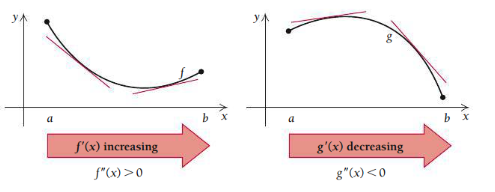
\includegraphics[width=0.7\textwidth]{ /home/mattw/niu/Math211/latexdocs/figures/ghg.png  }
\end{figure}
\subsection*{Concavity: Increasing and Decreasing Derivatives}
For the graph of $f$, the slopes of the tangent lines are increasing. That is, $f'$ is increasing over the interval. This can be determined by noting that $f''(x)$ is positive, since the relationship between $f'$ and $f''$ is like the relationship between $f$ and $f'$.
\bigbreak \noindent
For the graph of $g$, the slopes are decreasing. This can be determined by noting that $g'$ is decreasing whenever $g''(x)$ is negative. The bending of each curve is called the graphs \textbf{concavity}
\bigbreak \noindent
\begin{mdframed}
 Suppose that $f$ is a function whose derivative $f'$ exists at every point in an open interval $I$. Then 
\bigbreak \noindent
\hspace{26mm}$f$ is \textbf{concave up} on I if \hspace{31mm} $f$ is \textbf{concave down on I if}

\hspace{16mm}$f'$ is increasing over I \hspace{35mm} $f'$ is decreasing over I
\bigbreak
\hspace{30mm}\begin{minipage}{0.5\textwidth}
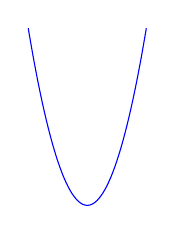
\begin{tikzpicture}
  \draw[scale=0.25,domain=-3:3,smooth,variable=\x,blue] plot ({\x},{\x*\x});
\end{tikzpicture}
\end{minipage}
\begin{minipage}{0.5\textwidth}
  \hspace{-20mm}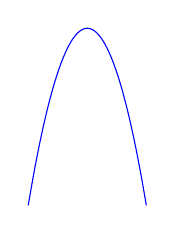
\begin{tikzpicture}
  \draw[scale=0.25,domain=-3:3,smooth,variable=\x,blue] plot ({\x},{-\x*\x});
\end{tikzpicture}
\end{minipage}
\end{mdframed}
\bigbreak \noindent
The following theorem states how concavity and the second derivative are related
\thm{}{
  \begin{enumerate}
    \item If $f''(x) > 0$ for all x on an open interval I, then the graph of $f$ is concave up on I
    \item If $f''(x) < 0$ for all x on an open interval I, then the graph of $f$ is concave down on I
  \end{enumerate}
}

\pagebreak
	
\noindent A function can be 
\begin{itemize}
  \item decreasing and concave up, 
\bigbreak \noindent
\item Decreasing and concave down,
\bigbreak \noindent
\item Increasing and concave up
\bigbreak \noindent
\item Or, increasing and concave down.
\end{itemize}
\bigbreak \noindent
  That is, \textbf{concavity}	and increasing/decreasing are seperate concepts. It is the increasing or decreasing aspect of the derivative that tells us about the functions concavity.
\begin{figure}[ht]
    \centering
    \incfig[1]{luh}
    %\caption{luh}
    %\label{fig:luh}
\end{figure}
\bigbreak \noindent
\subsection*{Classifying Relative Extrema Using Second Derivatives}
\thm{}{
  Suppose that $f$ is differentiable for every $x$ in an open interval (a,b) and that there is a critical value $c$ in (a,b) for which $f'(c) = 0$. Then:
  \begin{enumerate}
    \item $f(c) $ is a relative minimum if $f''(c) > 0$
    \item $f(c)$ is a relative maximum if $f''(c) < 0$
\bigbreak \noindent
  \end{enumerate}
 For $f''(c) = 0$, the First-Derivative Test can be used to determine whether $f(x)$ is a relative extremum
}
\pagebreak
\begin{mdframed}
\begin{minipage}{0.5\textwidth}
	\begin{tikzpicture}
\begin{axis}[
    xlabel={$x$},
    ylabel={$y$},
    axis lines=middle,
    xmin=-1, xmax=6,
    ymin=0, ymax=20,
    legend pos=middle,
]

\addplot[
    domain=-2:6,
    samples=100,
    smooth,
    thick,
    blue,
]{(x-2)^4 + 1};

\addlegendentry{$(x-2)^4 + 1$}
\end{axis}
\end{tikzpicture}
\end{minipage}
\begin{minipage}{0.5\textwidth}
	\begin{tikzpicture}
\begin{axis}[
    xlabel={$x$},
    ylabel={$y$},
    axis lines=middle,
    xmin=-1, xmax=6,
    ymin=-10, ymax=20,
    legend pos=north east,
    legend cell align={left},
]

\addplot[
    domain=-2:6,
    samples=100,
    smooth,
    thick,
    red,
]{(x-2)^3 + 1};

\addlegendentry{$(x-2)^3 + 1$}

\end{axis}
\end{tikzpicture}
\end{minipage}
\end{mdframed}
\bigbreak \noindent
Notice that the graph on the left has an extremum at c = 2 and the other function does not. In cases like this, An approach other than the Second-Derivative Test must be used to determine whether $f(c)$ is an extremum
\bigbreak \noindent
\q
Find any relative extrema and graph the function $f$ given by

$$ f(x) = x^3 + 3x^2 - 9x -13$$
\textit{\textbf{Take the first derivative}}

$$f'(x) = 3x^2 + 6x - 9$$
\bigbreak 
\noindent\textit{\textbf{To find any critical values, we solve $f'(x) = 0$}}
$$ 3x^2 + 6x-9= 0$$
$$ x^2 +2x-3=0$$
$$ (x+3)(x-1) = 0$$
$$ x = -3 \ \ \ or \ \ \ x = 1$$
\textit{\textbf{Sub the critical values in the original function}}
$$ f(-3) = (-3)^3 + 3(-3)^2 - 9(-3) -13 = 14$$
$$ f(1) = (1)^3 + 3(1)^2 - 9(1) -13 = -18$$
\textit{\textbf{Next, we find the second derivative}}
$$ f''(x) = 6x+6$$
\textit{\textbf{We use the Second-Derivative Test with the critical values}}
$$ f''(-3) = 6(-3) + 6 =-12 < 0$$
$$f''(1) = 6(1) + 6 =12 > 0$$
\bigbreak \noindent
Thus, $f(-3) = 14$ is a relative maximum and $f(1) = - 18$ is a relative minimum.
\bigbreak \noindent
We plot both $(-3,14)$ and $(1,-18)$, including short arcs at each point to indicate the concavity
\pagebreak
\begin{figure}[ht]
\centering
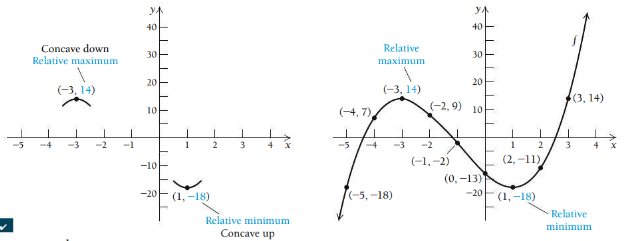
\includegraphics[width=0.9\textwidth]{ /home/mattw/niu/Math211/latexdocs/figures/concave.png }
\end{figure}
\q 
Find any relative extrema and graph the function $k$ given by
$$ k(x) = e^{2x} -e^x$$
\textit{\textbf{Take the first derivative}}
$$ k'(x) = 2e^{2x} - e^x$$
$$ e^x(2e^x - 1) = 0$$
$$ 2e^x - 1 = 0$$
$$ e^x  = \dfrac{1}{2}$$
\textit{\textbf{Take the natural log of both sides}}
$$ \ln{e^x} = \ln{\dfrac{1}{2}}$$
$$ x = \ln{0.5}$$
\textit{\textbf{Sub in the critical value into the original function}}
$$ k(\ln{0.5}) = e^{2(\ln{0.5})} - e^{\ln{0.5}}$$
$$ e^{\ln{0.5}^2} - e^{\ln{0.5}}$$
$$ = 0.5^2 - 0.5$$
$$ 0.25 - 0.5$$
$$ = -0.25$$
\textit{\textbf{Find the second derivative}}
$$ k''(x) = 4e^{2x} - e^x$$
$$ k''(\ln{0.5}) = 4e^{2(\ln0.5)} - e^{\ln0.5}$$
$$ 4e^{\ln0.5^2} - e^{\ln0.5}$$
$$ = 4(0.25) - 0.5$$
$$ = 0.5 > 0$$
Since the second derivative is positive at $\ln{0.5}$, we conclude that $k(\ln0.5) = -0.25$ is a relative minimum

\pagebreak
\begin{center}
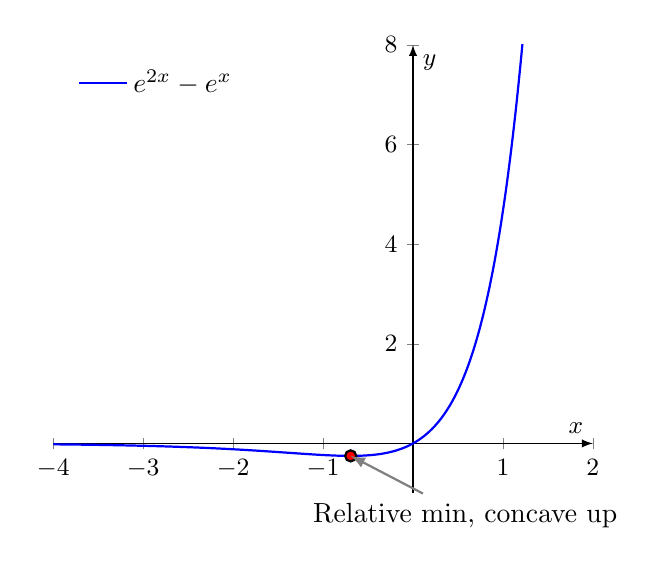
\begin{tikzpicture}
\begin{axis}[
    xlabel={$x$},
    ylabel={$y$},
    grid style=dashed,
    axis lines=center,
    axis line style=-latex,
    xmin=-4, xmax=2,
    ymin=-1, ymax=8,
    legend pos=north west,
    legend style={draw=none},
    clip mode=individual,
    every axis plot/.append style={thick},
    tick label style={font=\small},
    label style={font=\small},
]

\addplot[
    domain=-4:2,
    samples=100,
    smooth,
    blue,
    unbounded coords=jump,
]{exp(2*x) - exp(x)};
\addlegendentry{$e^{2x} - e^x$}

% Add a dot at the correct point (-ln(2), -1/4), which is approximately (-0.6931, -0.25)
\addplot[mark=*,mark options={fill=red}] coordinates {(-0.6931,-0.25)};

% Add annotation for relative min and concavity
\node[coordinate, pin={[pin distance=-1.2cm, pin edge={latex-,thick}]60:{Relative min, concave up}}] at (axis cs:-0.6931,-0.25) {};
\end{axis}
\end{tikzpicture}
\end{center}
\bigbreak \noindent
\subsection*{Points of Inflection}
A point at which concavity changes from down to up or from up to down is called a point of inflection, or an inflection point. In the figures below, point $P$ is an inflection point. The figures display the sign of $f''(x)$ to indicate the concavity on either side of $P$
\bigbreak \noindent
\begin{minipage}{0.3\textwidth}
    \incfig[1]{inf1}
\end{minipage}
\begin{minipage}{0.3\textwidth}
   \incfig[1]{incnine}
\end{minipage}
\begin{minipage}{0.3\textwidth}
    \incfig[1]{inceight}
\end{minipage}
\bigbreak \noindent
As we move along each curve, the concavity changes at $P$. Since the sign of $f''(x)$ changes, the value of $f''(x_0)$ at $P$ either must be 0 or must not exist.
\bigbreak \noindent
\thm{}{
  If $f$ has a point of inflection, it must occur at a value $x_0$, in the domain of $f$, where
  $$ f''(x_0)=0 \ \ \ or \ \ \ f''(x_0) \text{ does not exist}$$
}

\pagebreak
\q
Find the points of inflection on the graphs of
$$f(x) = x^3 + 3x^2 -9x-13$$
\textit{\textbf{Find the second derivative}}
$$ f''(x) = 6x +6$$
\textit{\textbf{Set equal to 0}}
$$ 6x + 6=0$$
$$ x = -1$$
\textit{\textbf{Test values on both intervals}}
$$ \text{Interval } (-\infty, -1): \ \ \ \text{Test } -2: \ \ \ f''(-2) = 6(-2) + 6 = -6 < 0$$
$$ \text{Interval } (-1,\infty): \ \ \ \text{Test } 0: \ \ \ f''(0) = 6(0) + 6 = 6 > 0$$
\bigbreak \noindent
$f$ is concave down on $(-\infty, -1)$
\bigbreak \noindent
$f$ is concave up on $(-1,\infty)$
\bigbreak \noindent
The sign of $f''(x)$ changes on either side of $x = -1$, so $(-1,-2)$ is a point of inflection
\nt{
  The first and second derivatives enhance our ability to sketch curves. We use the following strategy:
}
\begin{mdframed}
  \subsection*{Strategy for Sketching Graphs} 
  \bigbreak \noindent
 \item[(a)] \textbf{Derivatives and domain.} Find $f''(x)$ and $f'(x)$. Note the domain of $f$.
    
    \item[(b)] \textbf{Critical values of $f$.} Find the critical values by solving $f''(x) = 0$ and by finding where $f''(x)$ does not exist. These numbers yield candidates for relative maxima or minima. Find the function values at these points.
    
    \item[(c)] \textbf{Increasing and/or decreasing; relative extrema.} Substitute each critical value, $x_0$, from step (b) into $f'(x)$. If $f'(x_0) > 0$, then $f(x_0)$ is a relative maximum and $f$ is increasing on the left of $x_0$ and decreasing on the right. If $f'(x_0) < 0$, then $f(x_0)$ is a relative minimum and $f$ is decreasing on the left of $x_0$ and increasing on the right.
    
    \item[(d)] \textbf{Inflection points.} Determine candidates for inflection points by finding where $f'(x) = 0$ or where $f'(x)$ does not exist. Find the function values at any such points.
    
    \item[(e)] \textbf{Concavity.} Use any candidates for inflection points from step (d) to define intervals. Substitute test values into $f'(x)$ to determine where the graph is concave up $(f''(x) > 0)$ and where it is concave down $(f''(x) < 0)$. Step (c) may have provided some of this information.
    \item[(f)] \textbf{Sketch the graph.} Sketch the graph using the information from steps (a)–(e), plotting extra points as needed.
\end{mdframed}

\pagebreak
\q
Find any relative extrema and inflection points and graph
\bigbreak \noindent
\textit{\textbf{Take the first and second derivative and find the domains}}
$$f'(x) = 4x^3 - 4x$$
$$ f''(x) = 12x^2 - 4$$
The domain of $f$ $f'$ and $f''$ is $\mathbb{R}$
\bigbreak \noindent
\textit{\textbf{Find the critical values}}
$$ 4x^3 - 4x = 0$$
$$ 4x(x^2 - 1) = 0$$
$$ 4x = 0 \ \ \ or \ \ \ x^2 -1=0$$
$$x = 0 \ \ \ or \ \ \ x=\pm1$$
\textit{\textbf{find the critical points}}
$$ f(-1) = (-1,-1)$$
$$ f(0) = (0,0)$$
$$ f(1) = (1,-1)$$
\textit{\textbf{So, we have the intervals}}
$$ (-\infty, -1), (-1,0), (0,1), (1,\infty)$$
\textit{\textbf{Now we can find where the function is increasing and decreasing, as well as concavity and relative max and min by substituting the critical points into f''}}
$$f''(-1) = 8 > 0$$
Since $f''(-1) = 8 > 0$, we see that $f$ is decreasing on the left over then interval $(-\infty, -1)$ and increasing on $(-1,0)$, This shows us that $(-1,-1)$ is a relative min. And because the value we obtained from $f''(-1)$ is positive, it is also concave up
\textit{\textbf{Using the same logic for the other 2 critical values we get}}
$$ f''(0) = -4 < 0$$
So, $f$ is increasing over the interval $(-1,0)$, and decreasing over the interval $(0,1)$. It is a relative max, and concave down.
\bigbreak \noindent
$$ f''(1) = 8 > 0$$
So, $f$ is decreasing over the interval $(0,1)$, and increasing over the interval $(1,\infty)$. So, the critical point $(1,-1)$ is a relative min, and concave up
\bigbreak \noindent
\textit{\textbf{Next, we find the points of inflection by setting f'' equal to 0}}
$$ 12x^2 - 4 = 0$$
$$ 12x^2 = 4$$
$$ x^2 = \dfrac{1}{3}$$
$$ x = \pm\sqrt{\dfrac{1}{3}}$$

\pagebreak
\noindent \textit{\textbf{plug in these x values into the original function to find the y values}}
$$ f\left(\sqrt{\dfrac{1}{3}}\right) = \left(\sqrt{\dfrac{1}{3}}\right)^4 - 2 \left(\sqrt{\dfrac{1}{3}}\right)^2 = \dfrac{1}{9} - \dfrac{2}{3} = -\dfrac{5}{9}$$
$$ f\left(-\sqrt{\dfrac{1}{3}}\right) = \left(-\sqrt{\dfrac{1}{3}}\right)^4 - 2 \left(-\sqrt{\dfrac{1}{3}}\right)^2 = \dfrac{1}{9} - \dfrac{2}{3} = -\dfrac{5}{9}$$
So, our possible inflection points are
$$ \left(\sqrt{\dfrac{1}{3}}, -\dfrac{5}{9}\right) \left(-\sqrt{\dfrac{1}{3}}, -\dfrac{5}{9}\right)$$
So, Since the points of inflection are where the concavity switches, using the information obtained when we found concavity. We can conclude that $f$ is
\bigbreak \noindent
\begin{center}
Concave up on $\left(-\infty, -\sqrt{\dfrac{1}{3}}\right)$
\bigbreak \noindent
Concave down on $\left(-\sqrt{\dfrac{1}{3}}, \sqrt{\dfrac{1}{3}}\right)$
\bigbreak \noindent
Concave up on $\left(\sqrt{\dfrac{1}{3}}, \infty\right)$
\bigbreak \noindent
\end{center}
\begin{center}
\begin{tikzpicture}
\begin{axis}[
    xlabel={$x$},
    ylabel={$f(x)$},
    axis lines=center,
    width=15cm, % Set the width of the graph
    height=10cm, % Set the height of the graph
    xmin=-2.5, xmax=2.5,
    ymin=-3, ymax=6,
    domain=-2.5:2.5,
    samples=100,
    xlabel style={at={(ticklabel* cs:1)},anchor=north west},
    ylabel style={at={(ticklabel* cs:1)},anchor=south west}
]

% Add the function
\addplot [blue, thick] {x^4 - 2*x^2};
\addlegendentry{$f(x) = x^4 - 2x^2$}

% Add critical points
\addplot [only marks, mark=*, mark options={fill=red}, text mark as node=true] coordinates {(-1,-1) (0,0) (1,-1)};
\node[below right] at (axis cs:-1,-1) {\small $(-1,-1)$};
\node[above] at (axis cs:0,0) {\small $(0,0)$};
\node[below right] at (axis cs:1,-1) {\small $(1,-1)$};

% Add points of inflection
\addplot [only marks, mark=*, mark options={fill=green}, text mark as node=true] coordinates {(-0.577,-0.5555) (0.577,-0.5555)};
\node[above] at (axis cs:-0.577,-0.384) {\small $\left(-\sqrt{\dfrac{1}{3}},-\dfrac{5}{9}\right)$};
\node[above] at (axis cs:0.577,-0.384) {\small $\left(-\sqrt{\dfrac{1}{3}},-\dfrac{5}{9}\right)$};

\end{axis}
\end{tikzpicture}
\end{center}
\pagebreak
\section*{3.5 - Optimization: Business, Economics, and General Applications}
\q
\textbf{Maximizing Area.} The Hobby Farm has 20 ft of fencing to fence off a rectangular area for an electric train in one corner of its display room. The two sides up against the wall require no fence. What dimensions of the rectangle will maximize the area? What is the maximum area?
\bigbreak \noindent
\textit{\textbf{We let $x$ be the length of one side of the rectangle and $y$ the length of the other side. The area $A$ of the triangle formed by the fencing is given by the objective function.}}
$$ A = xy$$
\textit{\textbf{We are limited in the amount of fencing available: This is the constaint. Since 20 ft of fencing is available, the two side lengths $x$ and $y$ are related by the equation}}
$$ x + y =20, \ \ \ \text{or} \ \ \ y = 20-x$$
\begin{figure}[ht]
    \centering
    \incfig[1]{boxed}
    %\caption{boxed}
    %\label{fig:boxed}
\end{figure}
\bigbreak \noindent
The practical domain is $0\leq x\leq 20$, since the amount of fencing used for one side cannot be negative or greater than 20ft.
\bigbreak \noindent
$$8ft\cdot 12ft = 96ft^2$$
$$9ft \cdot 11ft = 99ft^2$$
$$ 10ft \cdot 10ft = 100ft^2$$
$$ 11ft \cdot 9ft = 99ft^2$$
$$ 12ft \cdot 8ft = 96ft^2$$
Based on this, it appears that letting $ x=10$ ft will result in a maxium area of 100ft$^2$. To be sure, we use calculus.
\bigbreak \noindent
Substituting the constraint $ y = 20 -x$ into the formula for area, we have
$$ A = xy$$
$$A=x(20-x)$$
$$A(x)=20x-2x$$
\textit{\textbf{Thus, we want to maximize}} 
$$A(x) = 20x-x^2 \text{ over} \ [0,20]$$
\textit{\textbf{We find $A'(x)$}}
$$A'(x) = 20-2x$$
\textit{\textbf{This derivative exists for all x in $(0,20)$. The only critical values are where $A'(x) = 0$}}
$$ 20 - 2x=0$$
$$ x = 10$$
$$\boxed{A(10) = 100}$$

\pagebreak
\noindent Thus, the point $(10,100)$ is a critical point on the graph of $A$. The student can confirm that, the endpoints $x=0$ and $x=20$ both result in a minimum area of $0$ft$^2$. We use the Second-Derivative Test to classify $(10,100)$ as a relative maximum or a relative minimum. The second derivative is
$$ A''(x) = -2$$
This means that the graph of $A$ is concave down for all x, so $(10,100)$ is a relative maximum point. By Maximum-Minimum Principle 1, we conclude that the \textit{absolute} maximum value of $A$ over the interval $[0,20]$ occurs at $x = 10$
\bigbreak \noindent
The Hobby Farm should use 10ft of fencing on one side and 10ft on the other, to achieve the largest possible area of 100ft$^2$. Using calculus has shown that this time, our original intuition of using 10 feet of fencing to a side was correct
\bigbreak \noindent \bigbreak \noindent
Here is a general strategy for solving maximum-minimum problems.
\bigbreak \noindent
\begin{mdframed}
  \subsection*{A Strategy for Solving Maximum-Minimum Problems}
  \begin{enumerate}
    \item Read the problem carefully. Make a drawing, and label any dimensions, if possible. 
    \item Make a list of appropriate variables and constraints, noting what varies, what stays fixed, and what units are being used. Label the measurements on your drawing.
      \item Translate the problem to an objective function $f$ that expresses the quantity to be maximized or minimized. Represent $f$ in terms of the varibles of step 2.
      \item Use algebra and Substitution as needed to express $f$ as a function of one variable
      \item Use the procedures developed in Sections 3.1-3.4 to determine the maximum or minimum values and the points at which they occur
  \end{enumerate}
\end{mdframed}
\bigbreak \noindent \bigbreak \noindent
\textbf{Maximizing Volume.} From a sheet of cardboard, 8in. by 11in., squares are cut out at the corners so that the sides can be folded up to make a box. What dimensions will yield a box of maximum volume? What is the maximum volume?
\bigbreak \noindent
\begin{minipage}{0.5\textwidth}
    \incfig[1]{cutbox}
\end{minipage}
\begin{minipage}{0.5\textwidth}
    \incfig[1]{cubed}
\end{minipage}
\bigbreak \noindent
After the four squares are removed and the sides are folded up, the volume $V$ of the resulting box is
$$ V = l \cdot w \cdot h = (11-2x) \cdot (8-2x) \cdot x$$

\pagebreak
\noindent
We have $V$ = $l\cdot w\cdot h = (11-2x) \cdot (8-2x) \cdot x$. Multiplying gives us the objective function.
$$ V(x) = 4x^3 - 38x^2 +88x$$
The amount cut out at each corner cannot be negative, nor can it be more than half of the 8-in. side length. Thus, the domain is
$$0\leq x \leq 4$$
Note that for x = 0 or x = 4, the volume is 0: In the first case, the box has no height, and in the second case, the box has no width.
\bigbreak \noindent
To determine critical values, we find $V'(x)$:
$$ V'(x) = 12x^2 - 76x + 88$$
Since $V'(x)$ is defined for all x in the interval (0,4), we set $V'(x) = 0$ to find any critical values. Using the quadratic formula, we have
$$ x = \dfrac{-(-76) \pm \sqrt{(-76)^2-4(12)(88)}}{2(12)} = \dfrac{76\pm\sqrt{1552}}{24}$$
Using a calculator and rounding to three decimal places, we have
$$ x  = \dfrac{76-\sqrt{1552}}{24}\approx 1.525 \ \ \ \text{and} \ \ \ x = \dfrac{76+\sqrt{1552}}{24}\approx 4.808$$
However, the second value is not in the domain of the objective function, so the only critical value is 1.525. Thus, the point
$$(1.525, V(1.525))$$
Is a critical point.
\bigbreak \noindent
To classify this critical point, we use the Second-Derivative Test. The second derivative is
$$ V''(x) = 24x-76$$
Evaluating at x = 1.525, we obtain
$$ V''(1.525) = 24(1.525) -76=-39.4 < 0$$
Since $V''(1.525)$ is negative, the graph of $V$ is concave down, indicating that $(1.525, V(1.525))$ is a relative maximum point over the interval [0,4]. Since we have already determined that both x = 0, and x = 4 (the endpoints) give zero volume, by Maximum-Minimum Principle 1, we conclude that $(1.525, V(1.525))$ must also be the \textbf{absolute} maximum point over [0,4]
\bigbreak \noindent
Thus, to maximize the volume of the box, we should cut a square of side length x = 1.525 in. from each corner, then fold up the flaps. The box will have a maximum volume of
$$ V(1.525) = 4(1.525)^3 - 38(1.525)^2 + 88(1.525) = 60.0126 \text{i n}^3$$

\pagebreak
\q
\textbf{Minimizing Cost of Material.} Mendoza Manufacturers specializes in food-storage containers and makes a cylindrical soup can with a volume of 250 cm$^3$. The cost of material for the two circular ends is \$0.0008/cm$^2$, and the cost of material for the side is \$0.0015/cm$^2$. What dimensions minimize the cost of material for the soup can? What is the minimum cost?

\end{document}


